Biomechanics researchers rely on numerical simulations of motion to gain understanding on a variety of scientific topics such as the physiological causes of movement disorders and their consequences on health [ref], the estimation of non-measurable physiological quantities [ref] and the optimality of human movement [ref].
The musculoskeletal models used in these simulations generally have a large number of degrees of freedom and they are governed by several ordinary differential equations (ODEs) which mainly implement multibody and muscle activation dynamics.
The complexity of these systems has led scientists to formulate their simulations as optimal control problems (OCP), relying on efficient non-linear optimization software to find trajectories that fulfil a desired task while enforcing the system dynamics and minimizing a cost (e.g. time of execution, energy expenditure, matching experimental data, etc.).
Up to very recently, there was no off-the-shelf software available to the community to quickly formulate and solve such musculoskeletal OCPs, leading researchers to develop their--often simplified--own solutions.

As a result, many approaches coexist to formulate and solve OCPs in the biomechanics literature. 
The formulation phase, also called transcription, consists in turning a specific trajectory optimization problem into a generic non-linear program (NLP) that will be
solved using a dedicated algorithm. 
A first family of so-called \textit{direct} transcription methods comes from numerical optimal control. 
They consist in straightforwardly choosing the state and/or the control as optimization variables at a given number of points along the trajectory and they rely on the integration of the system dynamics between these points. 
For instance, the direct collocation method has shown its efficiency in several studies investigating human motion [ref, à prendre dans papier MOCO]. 
It consists in approximating the integration of the system dynamics using polynomials that describe the state and control trajectories.
Its main advantages are that it leads to very sparse NLPs, that knowledge about the state trajectory can be used in the initialization, and that it handles unstable systems well \cite{diehl2006fast}. 
Its major disadvantage is that adaptive integration error control implies regridding the whole problem and thus changes the NLP dimensions, discarding its use for such application.
Direct multiple shooting is another direct method that was also applied with success in a lot of biomechanics [ref] and robotics [ref] studies.
Its advantages are mostly the same as for direct collocation in addition to combine integration error control with fixed NLP dimensions, as it relies on possibly adaptive ODE solvers to integrate the system dynamics.
Finally, simpler choices can be made, as in \cite{yeadon2000mechanics} [+ ref Begon], where the optimization variables are instants at which a switch in the motor strategy occurs, using polynomials function (4th, 5th order) in-between, or in \cite{leboeuf2006energetic} [+ ref  Huchez, Mowmbaur, McPhee, Opensim]], where the optimization variables are the coefficients of fourth order polynomial approximations of the states, with linking conditions to enforce the continuity of the controls. 
These last approaches are less generic than the direct methods as they either require a knowledge about the state and control trajectories that one often does not have when investigating complex biomechanics issues or ... 

\begin{figure}[t!]
\centering
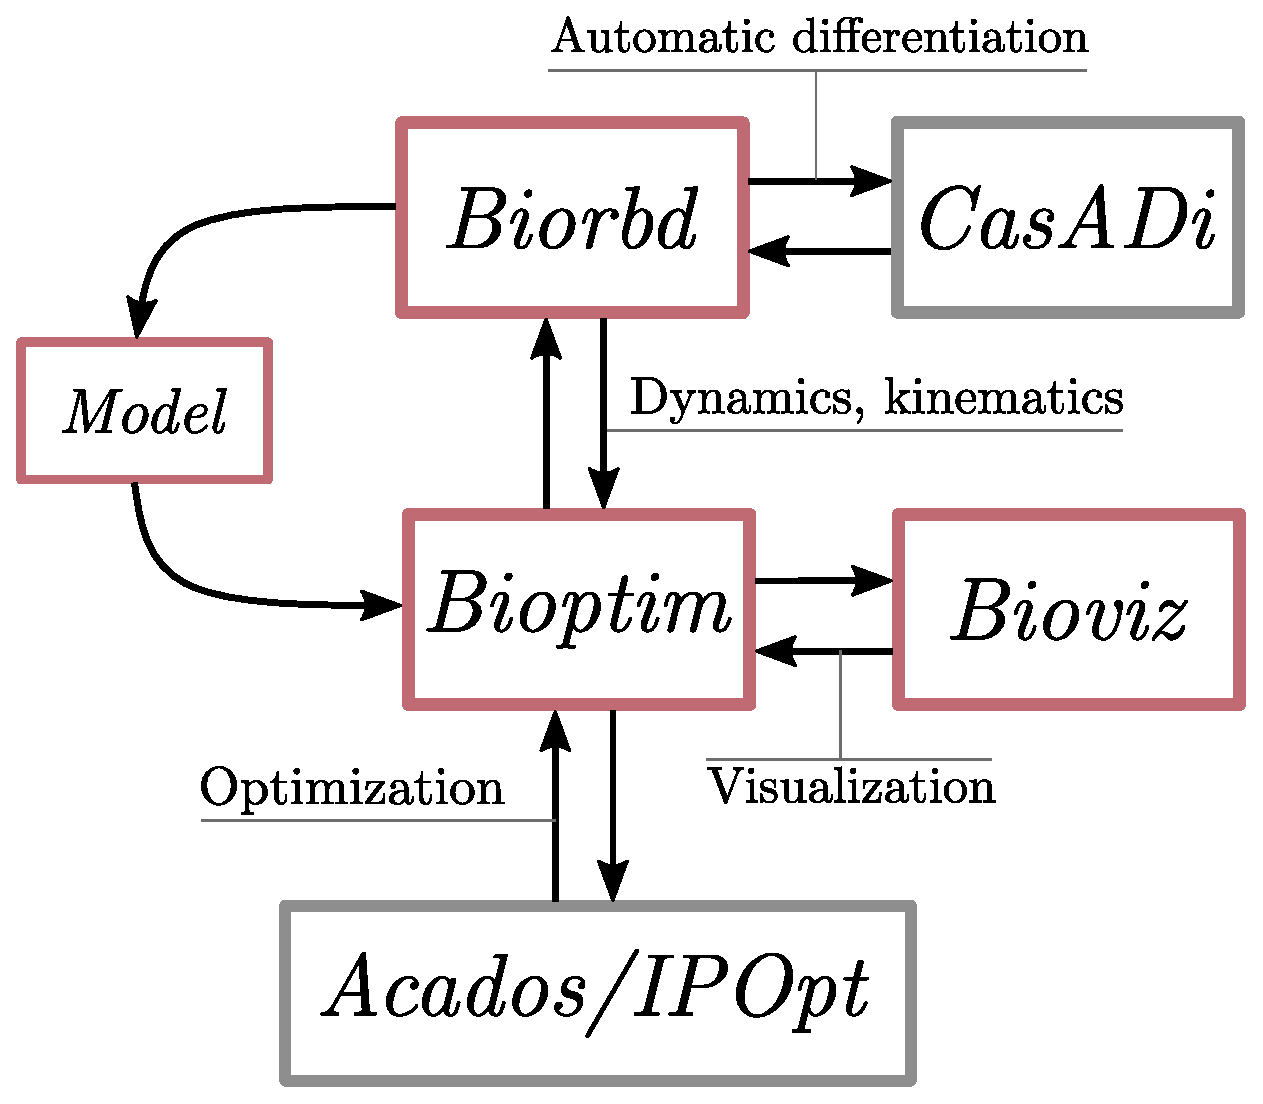
\includegraphics[width=0.9\columnwidth]{figures/dependencies.eps}
\caption{\bioptim dependencies flowchart. The red-boxed software are developed by the S2M team. The \bioptim part is further detailed in Fig.~\ref{fig:dependencies}.}
\label{fig:dependencies}
\vspace*{-0.5cm}
\end{figure}


In sports biomechanics, joint angle-driven algorithms are commonly implemented in which the joint angle time histories are approximated by series of quintic polynomial functions [REF Yeadon, Begon] or quartic splines [REF Leboeuf, Huchez, Mowmbaur, McPhee, Opensim]. 
Whereas evolutionary algorithms 
The number of papers about optimal control or dynamic optimisation is growing in robotics and biomechanics (Fig. X), probably because of increasing computer power but also the emergence of advanced open source (and proprietary) librairies for algorithmic differentiation and NLP solvers. 
Tools dedicated to OCP in biomechanics are rare. As shown by the recently launched MOCO, four interrelated components are required: \textit{i)} musculoskeletal modeling software (multibody kinematics and dynamics, muscle dynamics, etc.), \textit{ii)} a method for automatic differentiation, \textit{iii} a discretization approach, and \textit{iv)} a nonlinear programming (NLP) solver. Generic optimal control software (e.g. GPOPS-II [ref], Muscod-II [ref], Acado [ref]) provides solutions for component \textit{ii} to \textit{iv} but xxx. Since biomechanics is a community of software users [REFS], we believe that dedicated optimal control software will request a graphic user interface or at least a complete interface with a open source high-level language (e.g. Python) with a low-level core (C++) for efficiency. 

When developing such software, we should consider that human movements are often multi-staged (i.e. with different dynamics due to change in contact forces), [trouver d’autres], and models should be personalized, which may require several trials and parameter identification (e.g. isometric forces, mass properties of segments, etc.). 
Moreover, in contrast to the inverse flow which relies on measures, solving the ordinary differential equations (ODEs) of motion may result in unanticipated behaviours, ranging from non-physiological joint angles or muscle patterns to singularities. Either convenient constraints’ definition  and XXXXX\\ 

Lifting and relaxing OCPs\\ 
DMS et DC\\
Constraints vs cost\\


While CasADi is used in MOCO mainly for its interface to ipopt (ADOL-C being used for automatic differentiation),  this tool was first and foremost designed for algorithmic differentiation and is consequently widely used for solving NLP to reduce the cost and increase the accuracy of gradient and Hessian compared to finite-difference method. Acados, a recent NLP solver dedicated to DMS, was recently launched by the same research group as CasADi taking advantage of the algorithmic differentiation for real-time applications. Some applications, such as the real-time estimation of muscle forces, presently solved by inverse approach [REF] (from inverse dynamics to static optimization) or hybrid approach like the EMG-assisted algorithm in CEINMS [REF], become possible [citer article François-Amedeo].


The objective of the present paper is to introduce an innovative optimal control software for OCPs in biomechanics with the following features: 
Written in Python with 
Real-time capability 



The paper is organized as follow: 
